\documentclass{article}
\usepackage[utf8]{inputenc}
\usepackage[spanish]{babel}
\usepackage{listings}
\usepackage{graphicx}
\graphicspath{ {images/} }
\usepackage{cite}

\begin{document}

\begin{titlepage}
    \begin{center}
        \vspace*{1cm}
            
        \Huge
        \textbf{Ideas para el proyecto final - Informatica II.}
            
        \vspace{0.5cm}
        \LARGE
            
        \vspace{1.5cm}
            
        \textbf{Luis Miguel Gil Rodriguez.}
        \\
        \textbf{Maverick Sosa Tobon.}
        \vfill
        \vspace{0.8cm}
            
        \Large
        Despartamento de Ingeniería Electrónica y Telecomunicaciones\\
        Universidad de Antioquia\\
        Medellín\\
        Marzo de 2021
            
    \end{center}
\end{titlepage}
\tableofcontents
\newpage
\section{Sección introductoria} \label{intro}
En este documento, podremos encontrar la idea para desarrollar el proyecto final del curso de Informatica II, cabe mencionar que el juego que aquí plasmamos esta basado en un juego ya existente y en un futuro el proyecto será renombrado.
\section{Traffic Racer.} 
\subsection{Historia del Juego.}
Un conductor diestro en carreras clandestinas es emboscado por unos policías por lo que él procede a escapar, usando los mejores autos que estén a su disposición y esperando no ser atrapado.
\subsection{Jugabilidad.}
El usuario va a comenzar a avanzar mundo a mundo a través de una carretera de X metros, se planea que la distancia de cada mapa vaya incrementando. Al auto se le irá acabando la gasolina conforme va avanzando en el mapa, por lo que se distribuirán estratégicamente diferentes objetos de  tipo gasolina que cargue al 100% el tanque y el usuario pueda seguir avanzando. El usuario también podrá ir recolectando objetos tipo monedas con el objetivo de:
\begin{enumerate}
    \item Comprar autos.
    \item Cuando el usuario pierda un mapa, se le ofrecerá la posibilidad de revivir por una cantidad X de monedas.
\end{enumerate}
\begin{figure}[h]
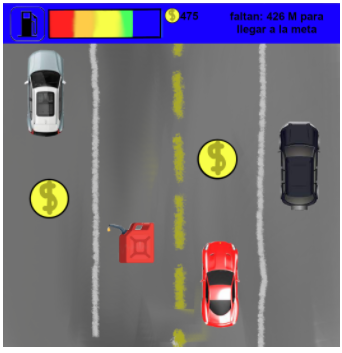
\includegraphics[width=6cm]{traffic_racer.PNG}
\centering
\caption{Mapa.}
\label{fig:mapa}
\end{figure}
\subsection{Dificultad.}
\begin{enumerate}
    \item Los autos (NPC) van a aparecer con mayot velocidad y frecuencia.
    \item Las monedas cada vez van a parecer más cerca de los NPC 's.
    \item La gasolina se va agotando y los bidones que recargan la gasolina aparecerán con menos frecuencia.
    \item Posibles huecos en la carretera.
\end{enumerate}
\subsection{¿Cómo se pierde un mapa?}
En el mapa se pierde cuando el nivel de gasolina llega a 0 Litros o cuando el jugador colisiona con uno de los carros/obstáculos que se encuentran en el mapa.
Cuando un mapa, aparecerá una imágen en donde estará él rodeado de autos de policía. 
\subsection{¿Cómo se planea que se vaya mermando el combustible a lo largo de cada mapa?}
Conforme se va avanzando en la historia del juego, lo más sensato es que la gasolina se vaya agotando más rápido en cada mapa, por ende eso se pretende solucionar por medio de funciones que dependan de la distancia recorrida y que cada vez tiendan a disminuir más rápido.
\subsection{Visión del jugador.}
Se planea que el usuario tenga una  perspectiva top-down del ambiente de juego (Vista cenital). A continuación encontraremos algunos ejemplos:
(Buscar en google: auto cenital png)
\\
Vista de algunos posibles autos:
\begin{figure}[h]
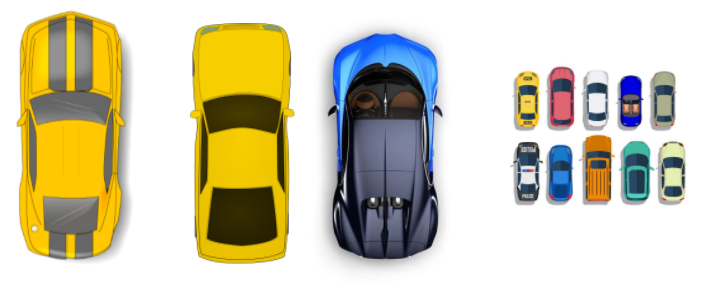
\includegraphics[width=6cm]{autos.PNG}
\centering
\caption{Autos.}
\label{fig:autos}
\end{figure}
Vista del posible escenario:
\begin{figure}[h]
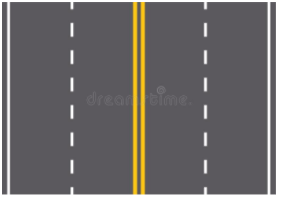
\includegraphics[width=6cm]{autopista.PNG}
\centering
\caption{Autopista.}
\label{fig:autopista}
\end{figure}
Gasolina:
\begin{figure}[h]
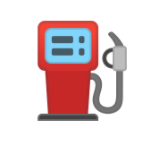
\includegraphics[width=6cm]{gasolina.PNG}
\centering
\caption{Gasolina.}
\label{fig:gasolina}
\end{figure}
Monedas:
\begin{figure}[h]

\includegraphics[width=6cm]{moneda.PNG}
\centering
\caption{Moneda.}
\label{fig:MOneda}
\end{figure}
En la parte superior de la pantalla se quiere mostrar cuantos metros faltan para llegar a la meta. el nivel actual de gasolina y la cantidad de monedas del usuario.
\subsection{¿Cómo se planea que el usuario guarde sus datos?}
Para eso se aplicará el manejo de archivos, para guardar el mapa en el que el usuario se encuentra, las monedas y autos con las que el usuario cuenta. Cada vez que el usuario termine satisfactoriamente un mapa o pierda un mapa se actualizará dicho archivo, al igual que cada que se compre un nuevo auto.
\subsection{Algunas clases que podemos utilizar.}
\begin{enumerate}
    \item Clase de gasolina.
    \item Clase Moneda.
    \item Clase Carros.
\end{enumerate}
\bibliographystyle{IEEEtran}
\bibliography{references}
\end{document}

